\chapter{Experimental Results}

In order to test the scalability and efficiency of the studied algorithms, the execution time was measured using only the \gls{gpu}, and while using only the \gls{cpu} and using both devices with a varying number of \gls{cpu} cores. The workload distribution between the devices was also measured by the DICE scheduler. Every time measurement was executed five times, selecting the best time as the final result. These tests were executed using the Living Room Scene with a resolution of 1024x768.

In order to evaluate the image quality produced by the studied algorithms, three scenes were used for testing, each with a different goal. The Sponza scene, courtesy of Crytek, is an outdoor scene with only diffuse materials, but complex geometry nonetheless. The Kitchen scene, courtesy of \todo[inline]{who to give credit to}, is an indoor scene with a lot of glossy materials. The final and most complex scene, the Living Room, courtesy of Iliyan Georgiev, is an indoor scene as well but with an emphasis on reflected caustics and complex lighting. For every scene a reference image was rendered with \gls{vcm} with 100000 samples per pixel. Then for every algorithm a set of images with an approximate rendering time were produced. All these images were compared to the reference image using the \gls{rmse} metric.

\begin{figure}[ht]
\centering
\begin{minipage}[b]{0.3\linewidth}
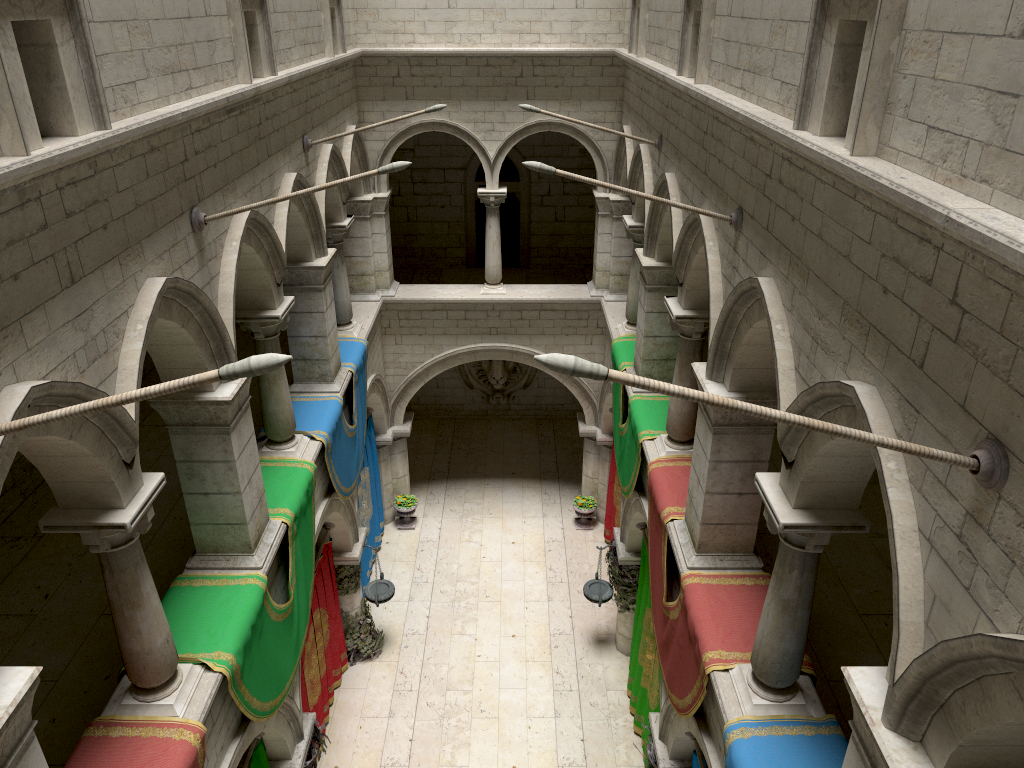
\includegraphics[width=\linewidth]{img/sponza_ref.jpg}
\caption{\label{img:sponza_ref} Sponza scene reference image.}
\end{minipage}
\quad
\begin{minipage}[b]{0.3\linewidth}
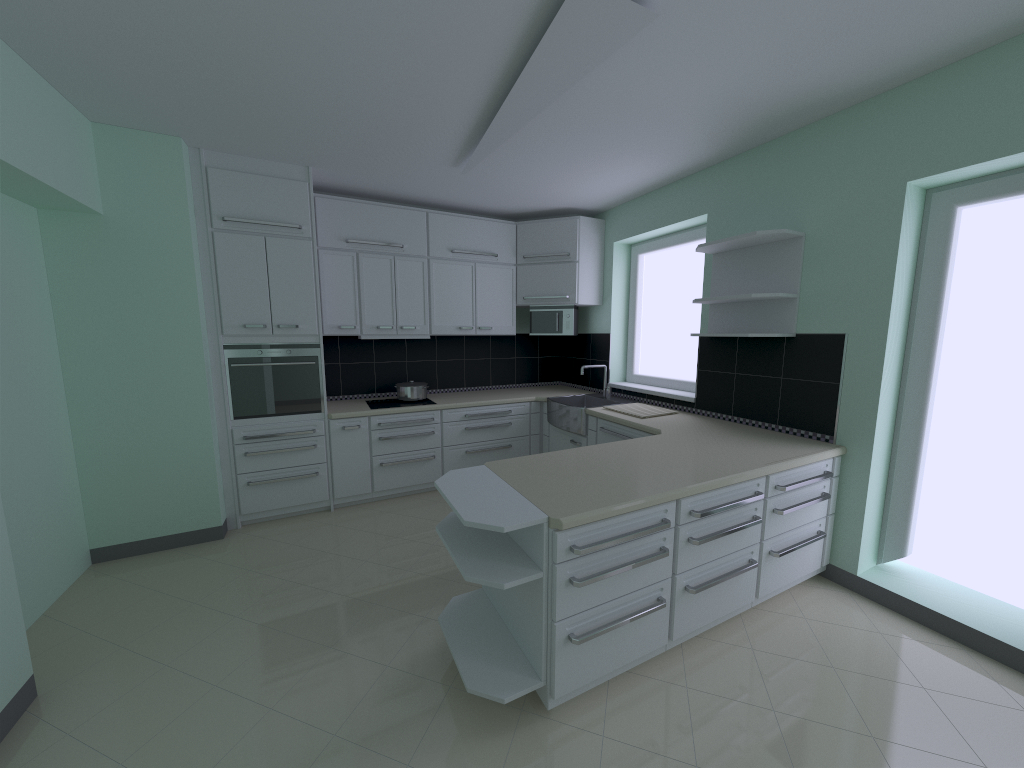
\includegraphics[width=\linewidth]{img/kitchen_ref.jpg}
\caption{\label{img:kitchen_ref} Kitchen scene reference image.}
\end{minipage}
\quad
\begin{minipage}[b]{0.3\linewidth}
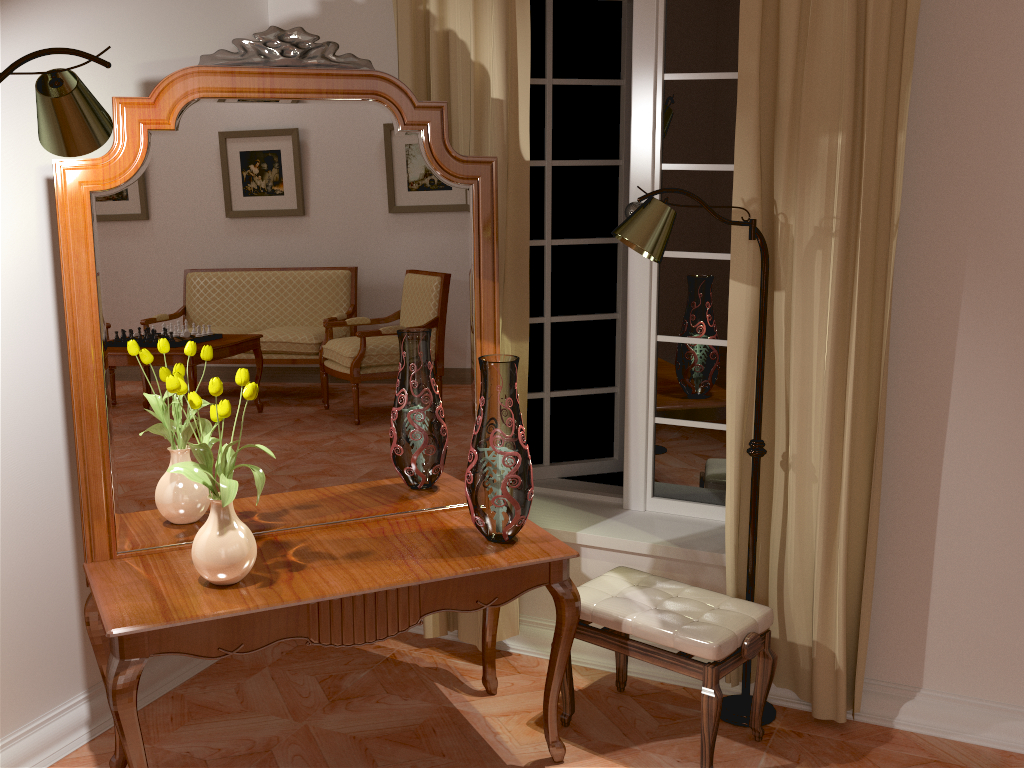
\includegraphics[width=\linewidth]{img/livingroom_ref.jpg}
\caption{\label{img:livingroom_ref} Living Room scene reference image.}
\end{minipage}

\end{figure}

\section{Setup}

All experiments were executed on a dual-socket computer with two 10 core Intel Xeon E5-2670 v2 \gls{cpu} at the frequency of 2.50GHz, 64 GB of RAM and a Nvidia Tesla K20 \gls{gpu}.

Every software used was updated to the versions listed in table~\ref{tab:soft_ver}.

\begin{table}[h]
\centering
\begin{tabular}{|l|l|}

\hline
Software & Version \\
\hline
Linux & 2.6.32-279 \\
\hline
GCC & 4.8.2 \\
\hline
CUDA Toolkit & 5.5 \\
\hline
Optix & 3.7 \\
\hline
Embree & 2.5.1 \\
\hline

\end{tabular}
\caption{\label{tab:soft_ver} Software Versions Used}
\end{table}


\section{Excution Time Results}

\begin{figure}[ht]
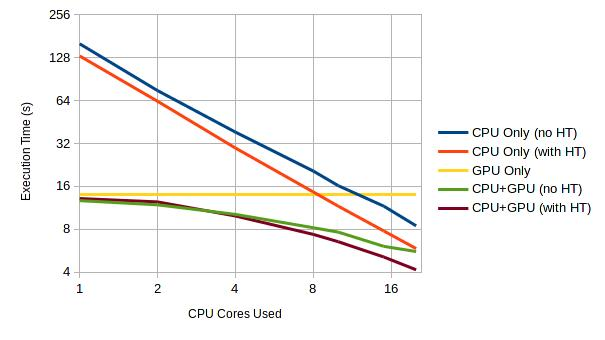
\includegraphics[width=\linewidth]{img/ptTexec.jpg}
\caption{\label{img:ptTexec} Path Tracer Execution Times}
\end{figure}

\begin{figure}[ht]
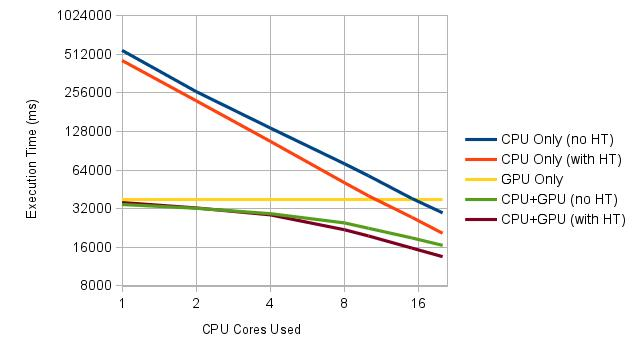
\includegraphics[width=\linewidth]{img/bptTexec.jpg}
\caption{\label{img:bptTexec} Bidirectional Path Tracer Execution Times}
\end{figure}

\begin{figure}[ht]
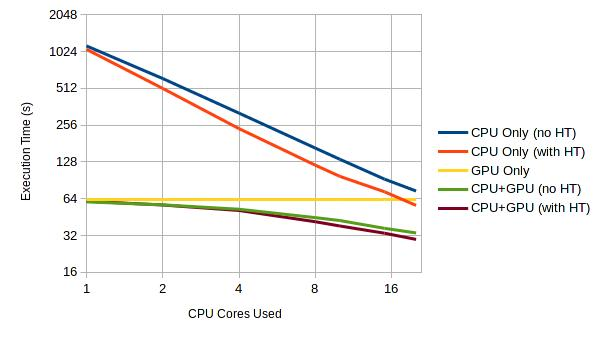
\includegraphics[width=\linewidth]{img/bpmTexec.jpg}
\caption{\label{img:bpmTexec} Bidirectional Photon Mapping Execution Times}
\end{figure}

\begin{figure}[ht]
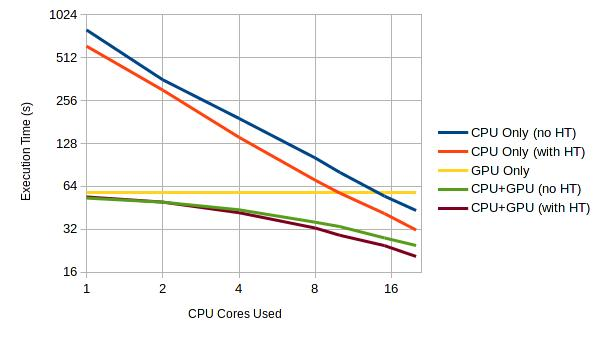
\includegraphics[width=\linewidth]{img/vcmTexec.jpg}
\caption{\label{img:vcmTexec} VCM Execution Times}
\end{figure}

\section{Speedup Results}